\documentclass[aspectratio=169,10pt]{beamer}

% Shared Beamer setup for Fall 2026 course slides.
% Clean Cal Poly-inspired theme: no custom class files or uncommon packages.
\mode<presentation>{
  \usetheme{default}
  \usefonttheme{professionalfonts}
}

\definecolor{CalPolyGreen}{HTML}{154734}
\definecolor{CalPolyGold}{HTML}{BD8B13}
\definecolor{CalPolySage}{HTML}{7FA28F}
\definecolor{CalPolyMint}{HTML}{DDF1E7}
\definecolor{CalPolySand}{HTML}{A29F86}
\definecolor{CalPolyBeige}{HTML}{EFEEDE}
\definecolor{DeckInk}{HTML}{1F2933}
\definecolor{DeckMuted}{HTML}{5F6B7A}
\definecolor{DeckSoft}{HTML}{F7F7F5}

\setbeamersize{text margin left=0.55in,text margin right=0.55in}
\setbeamercolor{normal text}{fg=DeckInk,bg=white}
\setbeamercolor{structure}{fg=CalPolyGreen}
\setbeamercolor{title}{fg=white}
\setbeamercolor{frametitle}{fg=CalPolyGreen,bg=white}
\setbeamercolor{block title}{bg=CalPolySage,fg=white}
\setbeamercolor{block body}{bg=CalPolyMint,fg=black}
\setbeamercolor{alerted text}{fg=CalPolyGold}

\setbeamerfont{title}{size=\Huge,series=\bfseries}
\setbeamerfont{frametitle}{size=\Large,series=\bfseries}
\setbeamerfont{block title}{size=\normalsize,series=\bfseries}

\setbeamertemplate{navigation symbols}{}
\setbeamertemplate{itemize item}{\color{CalPolyGold}$\blacktriangleright$}
\setbeamertemplate{itemize subitem}{\color{CalPolyGreen}$\bullet$}
\setbeamertemplate{footline}{
  \hfill{\color{DeckMuted}\scriptsize\insertframenumber/\inserttotalframenumber}
  \hspace{0.18in}\vspace{0.12in}
}
\setbeamertemplate{frametitle}{
  \vspace{0.18in}
  \hspace{0.02in}\insertframetitle\par
  \vspace{0.08in}
  \noindent\makebox[\linewidth][l]{%
    {\color{CalPolyGold}\rule{0.55in}{2pt}}%
    {\color{CalPolyGreen}\rule{\dimexpr\linewidth-0.55in\relax}{2pt}}%
  }
}

\newcommand{\CourseNumber}{Course}
\newcommand{\CourseTitle}{Course Title}
\newcommand{\LectureNumber}{0}
\newcommand{\LectureTitle}{Lecture Title}
\newcommand{\LectureDate}{Date}
\newcommand{\CourseUnit}{Unit}

\newcommand{\coursenumber}[1]{\renewcommand{\CourseNumber}{#1}}
\newcommand{\coursetitle}[1]{\renewcommand{\CourseTitle}{#1}}
\newcommand{\lecturenumber}[1]{\renewcommand{\LectureNumber}{#1}}
\newcommand{\lecturetitle}[1]{\renewcommand{\LectureTitle}{#1}}
\newcommand{\lecturedate}[1]{\renewcommand{\LectureDate}{#1}}
\newcommand{\courseunit}[1]{\renewcommand{\CourseUnit}{#1}}

\author{Kirk Duran}
\institute{California Polytechnic State University, San Luis Obispo}
\date{\LectureDate}

\newcommand{\makedecktitle}{
  \begingroup
  \setbeamercolor{background canvas}{bg=CalPolyGreen}
  \begin{frame}[plain]
    \vfill
    \begin{center}
      {\usebeamerfont{title}\color{white}\LectureTitle\par}
      \vspace{0.18in}
      {\Large\color{white}Lecture \LectureNumber\par}
    \end{center}
    \vfill
    \noindent{\color{white}\rule{\linewidth}{1.2pt}}\par
    \vspace{0.08in}
    \noindent\colorbox{CalPolyGold}{\makebox[0.24\linewidth][c]{\color{white}\Large\CourseNumber}}
    \hspace{0.12in}{\color{white}\Large Kirk Duran}
  \end{frame}
  \endgroup
}

\newenvironment{keyidea}{\begin{block}{Key idea}}{\end{block}}
\newenvironment{activity}{\begin{block}{In class}}{\end{block}}
\newenvironment{cpdefinition}{\begin{block}{Definition}}{\end{block}}
\newenvironment{exampleblockcp}{
  \begingroup
  \setbeamercolor{block title}{bg=CalPolySand,fg=white}
  \setbeamercolor{block body}{bg=CalPolyBeige,fg=black}
  \begin{block}{Example}
}{
  \end{block}
  \endgroup
}

\newcommand{\imageplaceholder}[2][0.3in]{%
  \noindent\makebox[\linewidth][c]{%
    \fcolorbox{CalPolySage}{CalPolyBeige}{%
      \parbox[c][#1][c]{0.86\linewidth}{%
        \centering
        {\color{DeckMuted}\scriptsize Image placeholder: }%
        {\color{DeckInk}\scriptsize\ttfamily\detokenize{#2}}%
      }%
    }%
  }%
}

\newcommand{\sectionframe}[1]{
  \begingroup
  \setbeamercolor{background canvas}{bg=CalPolyGreen}
  \begin{frame}[plain]
    \vfill
    {\color{white}\LARGE\bfseries #1\par}
    \vspace{0.18in}
    {\color{CalPolyGold}\rule{0.22\paperwidth}{3pt}}
    {\color{white}\rule{0.62\paperwidth}{3pt}}
    \vfill
  \end{frame}
  \endgroup
}

\newcommand{\placeholdernote}{
  \begin{block}{Placeholder}
    Replace these bullets with the final lecture material, examples, and in-class activities.
  \end{block}
}


\usepackage{tikz}
\usetikzlibrary{arrows.meta,shapes.geometric}

\pdfstringdefDisableCommands{\def\translate#1{#1}}

\graphicspath{{../assets/lecture-23/}}

% If an image file is not yet available, the slide displays a labeled
% placeholder using the intended filename. Place the matching file in
% ../assets/lecture-23/ to replace the placeholder automatically.
\newcommand{\lectureimage}[2][1.75in]{%
  \IfFileExists{../assets/lecture-23/#2}{%
    \includegraphics[width=\linewidth,height=#1,keepaspectratio]{#2}%
  }{%
    \fbox{%
      \parbox[c][#1][c]{0.94\linewidth}{%
        \centering
        \small\textbf{Image Placeholder}\\[0.08in]
        \scriptsize\texttt{\detokenize{#2}}
      }%
    }%
  }%
}

\setbeamersize{text margin left=0.42in,text margin right=0.42in}

\coursenumber{CS 1001}
\coursetitle{Introduction to Computing}
\lecturenumber{23}
\lecturetitle{Iteration II --- Common Loop Patterns}
\lecturedate{Fall 2026}
\courseunit{9. Iteration}

\begin{document}

\makedecktitle

\begin{frame}{Today}
  \begin{itemize}
    \item Recognize common patterns built from \texttt{for} loops.
    \item Use accumulators to compute totals and counts.
    \item Build new lists while preserving the original input.
    \item Select values conditionally during iteration.
    \item Choose between \texttt{for} and \texttt{while} loops.
    \item Trace \texttt{while} loops and spot termination and boundary bugs.
  \end{itemize}

  \begin{keyidea}
    Most useful loops are not arbitrary. They are instances of a small number of recurring computational patterns.
  \end{keyidea}
\end{frame}

\sectionframe{Part 1: From Individual Loops to Patterns}



\begin{frame}{A Pattern Has Four Parts}
  Many loops can be understood using four questions.

  \begin{enumerate}
    \item \textbf{Initialization:} What state exists before the loop begins?
    \item \textbf{Iteration:} What values are examined?
    \item \textbf{Update:} How does the state change during each iteration?
    \item \textbf{Result:} What value is used after the loop finishes?
  \end{enumerate}

  \begin{block}{Example questions}
    Is the state an integer count? A running total? A new list being constructed?
  \end{block}
\end{frame}

\begin{frame}{Same Loop Structure, Different Computation}
  \begin{columns}[T,onlytextwidth]
    \begin{column}{0.46\textwidth}
      \begin{block}{Running total}
        \texttt{total = 0}\\
        \texttt{for value in values:}\\
        \hspace{0.18in}\texttt{total = total + value}
      \end{block}
    \end{column}
    \begin{column}{0.46\textwidth}
      \begin{block}{Counting matches}
        \texttt{count = 0}\\
        \texttt{for value in values:}\\
        \hspace{0.18in}\texttt{if value > 0:}\\
        \hspace{0.36in}\texttt{count = count + 1}
      \end{block}
    \end{column}
  \end{columns}

  The control structure is similar. The \textbf{meaning of the changing state} is different.
\end{frame}



\sectionframe{Part 2: Accumulation and Counting}

\begin{frame}{Pattern 1: Accumulating a Total}
  \begin{block}{Function}
    \texttt{def tally(nums: list[int]) -> int:}\\
    \hspace{0.20in}\texttt{total = 0}\\
    \hspace{0.20in}\texttt{for num in nums:}\\
    \hspace{0.40in}\texttt{total = total + num}\\
    \hspace{0.20in}\texttt{return total}
  \end{block}

  \begin{center}
    \renewcommand{\arraystretch}{1.25}
    \begin{tabular}{l|l}
      \textbf{Role} & \textbf{Code} \\\hline
      initialize & \texttt{total = 0} \\
      iterate & \texttt{for num in nums} \\
      update & \texttt{total = total + num} \\
      result & \texttt{return total}
    \end{tabular}
  \end{center}
\end{frame}

\begin{frame}{Trace the Running Total}
  For \texttt{tally([4, 9, 2, 1])}:

  \begin{center}
    \renewcommand{\arraystretch}{1.3}
    \begin{tabular}{c|c|c|c}
      \textbf{Iteration} & \textbf{\texttt{num}} & \textbf{\texttt{total} before} & \textbf{\texttt{total} after} \\\hline
      1 & 4 & 0 & 4 \\
      2 & 9 & 4 & 13 \\
      3 & 2 & 13 & 15 \\
      4 & 1 & 15 & 16
    \end{tabular}
  \end{center}

  \begin{keyidea}
    The value computed during one iteration becomes part of the starting state for the next iteration.
  \end{keyidea}
\end{frame}



\begin{frame}{Pattern 2: Counting}
  Counting is another accumulator pattern.

  \begin{block}{Count positive values}
    \texttt{count = 0}\\
    \texttt{for value in values:}\\
    \hspace{0.20in}\texttt{if value > 0:}\\
    \hspace{0.40in}\texttt{count = count + 1}
  \end{block}

  The accumulator does not store the values themselves. It stores \textbf{how many} values satisfy a condition.
\end{frame}

\begin{frame}{Conditional Updates}
  Suppose:

  \begin{block}{Code}
    \texttt{values = [-2, 5, 0, 7]}\\
    \texttt{count = 0}\\
    \texttt{for value in values:}\\
    \hspace{0.20in}\texttt{if value > 0:}\\
    \hspace{0.40in}\texttt{count = count + 1}
  \end{block}

  \begin{center}
    \renewcommand{\arraystretch}{1.25}
    \begin{tabular}{c|c|c|c}
      \textbf{Iteration} & \textbf{value} & \textbf{\texttt{value > 0}} & \textbf{count after} \\\hline
      1 & -2 & False & 0 \\
      2 & 5 & True & 1 \\
      3 & 0 & False & 1 \\
      4 & 7 & True & 2
    \end{tabular}
  \end{center}
\end{frame}



\begin{frame}{Counting Characters in a String}
  The same pattern works with strings.

  \begin{block}{Function}
    \texttt{def count\_a(text: str) -> int:}\\
    \hspace{0.20in}\texttt{count = 0}\\
    \hspace{0.20in}\texttt{for char in text:}\\
    \hspace{0.40in}\texttt{if char == "a":}\\
    \hspace{0.60in}\texttt{count = count + 1}\\
    \hspace{0.20in}\texttt{return count}
  \end{block}

  \texttt{count\_a("banana")} returns \texttt{3}.
\end{frame}

\begin{frame}{Trace \texttt{count\_a("banana")}}
  \begin{center}
    \renewcommand{\arraystretch}{1.22}
    \begin{tabular}{c|c|c|c}
      \textbf{Iteration} & \textbf{char} & \textbf{\texttt{char == "a"}} & \textbf{count after} \\\hline
      1 & b & False & 0 \\
      2 & a & True & 1 \\
      3 & n & False & 1 \\
      4 & a & True & 2 \\
      5 & n & False & 2 \\
      6 & a & True & 3
    \end{tabular}
  \end{center}

  The pattern is unchanged even though the sequence type is different.
\end{frame}

\begin{frame}{Accumulator vs. Loop Variable}
  These names have different roles.

  \begin{center}
    \renewcommand{\arraystretch}{1.3}
    \begin{tabular}{l|l}
      \textbf{Name} & \textbf{Role} \\\hline
      \texttt{char} & rebound to the next sequence element \\
      \texttt{count} & stores state accumulated across iterations
    \end{tabular}
  \end{center}

  \begin{alertblock}{Common confusion}
    The loop variable normally changes because the loop rebinds it. The accumulator changes because the loop body explicitly assigns a new value to it.
  \end{alertblock}
\end{frame}

\begin{frame}{Bug: Initializing Inside the Loop}
  \begin{columns}[T,onlytextwidth]
    \begin{column}{0.47\textwidth}
      \begin{block}{Incorrect}
        \texttt{for value in values:}\\
        \hspace{0.18in}\texttt{total = 0}\\
        \hspace{0.18in}\texttt{total = total + value}
      \end{block}
    \end{column}
    \begin{column}{0.47\textwidth}
      \begin{block}{Correct}
        \texttt{total = 0}\\
        \texttt{for value in values:}\\
        \hspace{0.18in}\texttt{total = total + value}
      \end{block}
    \end{column}
  \end{columns}

  \begin{keyidea}
    If the accumulator is reinitialized during every iteration, earlier progress is discarded.
  \end{keyidea}
\end{frame}

\begin{frame}{Bug: Returning Too Early}
  \begin{block}{Incorrect}
    \texttt{def tally(nums: list[int]) -> int:}\\
    \hspace{0.20in}\texttt{total = 0}\\
    \hspace{0.20in}\texttt{for num in nums:}\\
    \hspace{0.40in}\texttt{total = total + num}\\
    \hspace{0.40in}\texttt{return total}
  \end{block}

  The first \texttt{return} ends the function call immediately.

  \begin{alertblock}{Consequence}
    For a non-empty input, only the first element is processed.
  \end{alertblock}
\end{frame}

\sectionframe{Part 3: Building New Lists}

\begin{frame}{Pattern 3: Build a New List}
  Some loops accumulate a \textbf{list} rather than a number.

  \begin{block}{General shape}
    \texttt{result = []}\\
    \texttt{for value in values:}\\
    \hspace{0.20in}\texttt{result.append(...)}\\
    \texttt{return result}
  \end{block}

  \begin{keyidea}
    The new list is the accumulator. Each iteration intentionally mutates that result list by appending another element.
  \end{keyidea}
\end{frame}

\begin{frame}{Copying with a Loop}
  \begin{block}{Function}
    \texttt{def copy(nums: list[int]) -> list[int]:}\\
    \hspace{0.20in}\texttt{new\_list = []}\\
    \hspace{0.20in}\texttt{for idx in range(len(nums)):}\\
    \hspace{0.40in}\texttt{new\_list.append(nums[idx])}\\
    \hspace{0.20in}\texttt{return new\_list}
  \end{block}

  The input is read. The new list is mutated.

  \begin{center}
    \texttt{new\_list is nums} is \texttt{False}, even when their contents are equal.
  \end{center}
\end{frame}

\begin{frame}{Trace the New List}
  For \texttt{copy([4, 9, 2, 1])}:

  \begin{center}
    \renewcommand{\arraystretch}{1.22}
    \begin{tabular}{c|c|c|l}
      \textbf{Iteration} & \textbf{idx} & \textbf{\texttt{nums[idx]}} & \textbf{new\_list after} \\\hline
      1 & 0 & 4 & \texttt{[4]} \\
      2 & 1 & 9 & \texttt{[4, 9]} \\
      3 & 2 & 2 & \texttt{[4, 9, 2]} \\
      4 & 3 & 1 & \texttt{[4, 9, 2, 1]}
    \end{tabular}
  \end{center}

  The result grows one element at a time.
\end{frame}

\begin{frame}{Intentional Mutation vs. Unintended Mutation}
  In a list-building function, this is intentional:

  \begin{block}{Intentional}
    \texttt{new\_list = []}\\
    \texttt{new\_list.append(value)}
  \end{block}

  This would change the caller's list instead:

  \begin{block}{Different behavior}
    \texttt{new\_list = nums}\\
    \texttt{new\_list.append(value)}
  \end{block}

  \begin{keyidea}
    The critical design question is \emph{which list is supposed to change?}
  \end{keyidea}
\end{frame}

\begin{frame}{Pattern 4: Transform Every Value}
  A common pattern is to produce one new value for every input value.

  \begin{block}{Function}
    \texttt{def increment\_all(nums: list[int]) -> list[int]:}\\
    \hspace{0.20in}\texttt{new\_list = []}\\
    \hspace{0.20in}\texttt{for value in nums:}\\
    \hspace{0.40in}\texttt{new\_list.append(value + 1)}\\
    \hspace{0.20in}\texttt{return new\_list}
  \end{block}

  Input and output have the same number of elements, but corresponding values differ.
\end{frame}

\begin{frame}{Trace the Transformation}
  For \texttt{increment\_all([4, 9, 2, 1])}:

  \begin{center}
    \renewcommand{\arraystretch}{1.25}
    \begin{tabular}{c|c|c|l}
      \textbf{Iteration} & \textbf{value} & \textbf{value + 1} & \textbf{new\_list after} \\\hline
      1 & 4 & 5 & \texttt{[5]} \\
      2 & 9 & 10 & \texttt{[5, 10]} \\
      3 & 2 & 3 & \texttt{[5, 10, 3]} \\
      4 & 1 & 2 & \texttt{[5, 10, 3, 2]}
    \end{tabular}
  \end{center}
\end{frame}





\sectionframe{Part 4: Selecting Values During Iteration}

\begin{frame}{Pattern 5: Build a List Conditionally}
  Sometimes only some input values belong in the result.

  \begin{block}{Positive values}
    \texttt{result = []}\\
    \texttt{for value in nums:}\\
    \hspace{0.20in}\texttt{if value > 0:}\\
    \hspace{0.40in}\texttt{result.append(value)}
  \end{block}

  The loop examines every value. The conditional decides whether the result list changes.
\end{frame}

\begin{frame}{Trace Conditional List Building}
  For \texttt{[-3, 5, 0, -1, 8, 2]}:

  \begin{center}
    \renewcommand{\arraystretch}{1.16}
    \begin{tabular}{c|r|c|l}
      \textbf{Iteration} & \textbf{value} & \textbf{\texttt{value > 0}} & \textbf{result after} \\\hline
      1 & -3 & False & \texttt{[]} \\
      2 & 5 & True & \texttt{[5]} \\
      3 & 0 & False & \texttt{[5]} \\
      4 & -1 & False & \texttt{[5]} \\
      5 & 8 & True & \texttt{[5, 8]} \\
      6 & 2 & True & \texttt{[5, 8, 2]}
    \end{tabular}
  \end{center}
\end{frame}

\begin{frame}{Counting vs. Collecting}
  These patterns may use the same condition but produce different results.

  \begin{columns}[T,onlytextwidth]
    \begin{column}{0.46\textwidth}
      \begin{block}{Count matches}
        \texttt{count = 0}\\
        \texttt{for value in nums:}\\
        \hspace{0.18in}\texttt{if value > 0:}\\
        \hspace{0.36in}\texttt{count += 1}
      \end{block}
    \end{column}
    \begin{column}{0.46\textwidth}
      \begin{block}{Collect matches}
        \texttt{result = []}\\
        \texttt{for value in nums:}\\
        \hspace{0.18in}\texttt{if value > 0:}\\
        \hspace{0.36in}\texttt{result.append(value)}
      \end{block}
    \end{column}
  \end{columns}

  One result is an integer. The other is a list.
\end{frame}

\begin{frame}{Transforming Only Selected Values}
  We can combine a condition with a transformation.

  \begin{block}{Code}
    \texttt{result = []}\\
    \texttt{for value in values:}\\
    \hspace{0.20in}\texttt{if value > 0:}\\
    \hspace{0.40in}\texttt{result.append(value * 2)}
  \end{block}

  Example:
  \begin{center}
    \texttt{[-1, 3, 0, 5]} $\rightarrow$ \texttt{[6, 10]}
  \end{center}

  \begin{keyidea}
    The condition determines \emph{which} values contribute. The expression determines \emph{what} each contribution becomes.
  \end{keyidea}
\end{frame}



\begin{frame}{Trace Two Accumulators at Once}
  For \texttt{values = [-1, 3, 0, 5]}:

  \begin{center}
    \renewcommand{\arraystretch}{1.2}
    \begin{tabular}{c|r|c|c|l}
      \textbf{Iter.} & \textbf{value} & \textbf{positive?} & \textbf{total} & \textbf{output} \\\hline
      1 & -1 & False & 0 & \texttt{[]} \\
      2 & 3 & True & 3 & \texttt{[6]} \\
      3 & 0 & False & 3 & \texttt{[6]} \\
      4 & 5 & True & 8 & \texttt{[6, 10]}
    \end{tabular}
  \end{center}

  \begin{activity}
    Which values determine control flow? Which variables preserve state across iterations?
  \end{activity}
\end{frame}


\sectionframe{Part 5: While Loops and Their Pitfalls}

\begin{frame}[t]{A While Loop Repeats While a Condition Is True}
  \small
  A \texttt{for} loop takes successive items from an iterable. A \texttt{while} loop tests a condition before each iteration.
  \begin{columns}[T,onlytextwidth]
    \begin{column}{0.45\textwidth}
      \begin{block}{General shape}
        \texttt{initialize state}\\
        \texttt{while condition:}\\
        \hspace{0.18in}\texttt{do work}\\
        \hspace{0.18in}\texttt{update state}
      \end{block}
    \end{column}
    \begin{column}{0.50\textwidth}
      \begin{block}{Countdown}
        \texttt{remaining = 3}\\
        \texttt{while remaining > 0:}\\
        \hspace{0.18in}\texttt{print(remaining)}\\
        \hspace{0.18in}\texttt{remaining = remaining - 1}\\
        \texttt{print("Go!")}
      \end{block}
    \end{column}
  \end{columns}
  Output: \texttt{3}, \texttt{2}, \texttt{1}, then \texttt{Go!}, each on its own line.
  \begin{keyidea}
    The condition controls repetition. The body must make progress toward stopping when termination is intended.
  \end{keyidea}
\end{frame}

\begin{frame}[t]{Follow the Condition Back Around the Loop}
  \small
  \begin{center}
    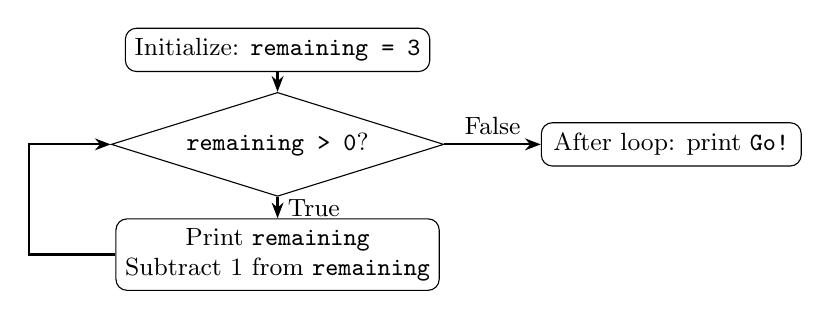
\begin{tikzpicture}[x=1cm,y=1cm,
      loopbox/.style={draw,rounded corners,align=center,minimum width=3.3cm,minimum height=0.55cm,font=\small},
      link/.style={-{Stealth[length=2mm]},thick}]
      \node[loopbox] (init) at (0,2.4) {Initialize: \texttt{remaining = 3}};
      \node[draw,diamond,aspect=3.2,align=center,font=\small] (test) at (0,1.2) {\texttt{remaining > 0}?};
      \node[loopbox] (body) at (0,-0.2) {Print \texttt{remaining}\\Subtract 1 from \texttt{remaining}};
      \node[loopbox] (done) at (5,1.2) {After loop: print \texttt{Go!}};
      \draw[link] (init)--(test);
      \draw[link] (test)--node[right,font=\small]{True} (body);
      \draw[link] (test)--node[above,font=\small]{False} (done);
      \draw[link] (body.west) -- ++(-1.1,0) |- (test.west);
    \end{tikzpicture}
  \end{center}
  \begin{keyidea}
    Test before the first iteration and again after each complete body. An initially false condition means zero iterations.
  \end{keyidea}
\end{frame}

\begin{frame}[t]{Trace the Final False Test Too}
  \small
  For the countdown starting at \texttt{remaining = 3}:
  \begin{center}
    \renewcommand{\arraystretch}{1.35}
    \begin{tabular}{c|c|c|l|c}
      \textbf{Test} & \textbf{remaining} & \textbf{remaining > 0} & \textbf{Body output} & \textbf{After body}\\\hline
      1 & 3 & True & \texttt{3} & 2\\
      2 & 2 & True & \texttt{2} & 1\\
      3 & 1 & True & \texttt{1} & 0\\
      4 & 0 & False & none; exit loop & 0
    \end{tabular}
  \end{center}
  Four condition tests, three body executions. After the loop, \texttt{print("Go!")} runs once.
  \begin{activity}
    What if \texttt{remaining} starts at \texttt{0}? The body never runs; the program prints only \texttt{Go!}.
  \end{activity}
\end{frame}

\begin{frame}[t]{For vs. While: Choose by What Controls Repetition}
  \small
  \begin{columns}[T,onlytextwidth]
    \begin{column}{0.46\textwidth}
      \begin{block}{For: consume items}
        \texttt{for step in range(3):}\\
        \hspace{0.18in}\texttt{print(step)}
      \end{block}
      Prefer this when visiting items in a list or string, or repeating over a range. Python advances the iterator for you.
    \end{column}
    \begin{column}{0.49\textwidth}
      \begin{block}{While: test a condition}
        \texttt{step = 0}\\
        \texttt{while step < 3:}\\
        \hspace{0.18in}\texttt{print(step)}\\
        \hspace{0.18in}\texttt{step = step + 1}
      \end{block}
      Prefer this when stopping depends on changing state, such as a user's next response. Manage progress explicitly.
    \end{column}
  \end{columns}
  Both examples print \texttt{0}, \texttt{1}, \texttt{2}.
  \begin{keyidea}
    These forms can express the same computation. Choose the one that makes the stopping rule clearest; a \texttt{for} loop need not know the item count in advance.
  \end{keyidea}
\end{frame}

\begin{frame}[t]{Use While When the User Decides When to Stop}
  \small
  Read commands until the user types exactly \texttt{quit}:
  \begin{block}{Sentinel-controlled input}
    \texttt{command = input("Command (quit to stop): ")}\\
    \texttt{while command != "quit":}\\
    \hspace{0.20in}\texttt{print("You entered:", command)}\\
    \hspace{0.20in}\texttt{command = input("Command (quit to stop): ")}\\
    \texttt{print("Done")}
  \end{block}
  \begin{itemize}
    \item \texttt{quit} is the \textbf{sentinel}: a special value meaning stop.
    \item The first input initializes the state; the input inside the body refreshes it.
  \end{itemize}
  \begin{keyidea}
    Future input determines when this stops. Without another input call, the condition keeps checking the old command.
  \end{keyidea}
\end{frame}

\begin{frame}[t]{Pitfall: No Progress Toward a False Condition}
  \small
  Both examples below keep the condition true indefinitely:
  \begin{columns}[T,onlytextwidth]
    \begin{column}{0.46\textwidth}
      \begin{alertblock}{Missing update}
        \texttt{remaining = 3}\\
        \texttt{while remaining > 0:}\\
        \hspace{0.18in}\texttt{print(remaining)}
      \end{alertblock}
      \texttt{remaining} stays at \texttt{3}.
    \end{column}
    \begin{column}{0.49\textwidth}
      \begin{alertblock}{Wrong direction}
        \texttt{remaining = 3}\\
        \texttt{while remaining > 0:}\\
        \hspace{0.18in}\texttt{remaining = remaining + 1}
      \end{alertblock}
      \texttt{remaining} grows: \texttt{4}, \texttt{5}, \texttt{6}, \ldots
    \end{column}
  \end{columns}
  Fix the countdown with \texttt{remaining = remaining - 1} inside the loop.
  \begin{keyidea}
    Check every path through the body: does the state change so the condition can eventually become false? If a loop is stuck, interrupt it with Stop or Ctrl+C, then inspect the condition and updates.
  \end{keyidea}
\end{frame}

\begin{frame}[t]{Pitfall: A Conditional Update Can Get Stuck}
  \small
  \begin{columns}[T,onlytextwidth]
    \begin{column}{0.47\textwidth}
      \begin{alertblock}{Incorrect}
        \texttt{i = 0}\\
        \texttt{while i < 3:}\\
        \hspace{0.18in}\texttt{if i > 0:}\\
        \hspace{0.36in}\texttt{print(i)}\\
        \hspace{0.36in}\texttt{i = i + 1}
      \end{alertblock}
    \end{column}
    \begin{column}{0.47\textwidth}
      \begin{block}{Correct}
        \texttt{i = 0}\\
        \texttt{while i < 3:}\\
        \hspace{0.18in}\texttt{if i > 0:}\\
        \hspace{0.36in}\texttt{print(i)}\\
        \hspace{0.18in}\texttt{i = i + 1}
      \end{block}
    \end{column}
  \end{columns}
  On the left, \texttt{i > 0} is false at \texttt{i = 0}, so neither statement runs. The next iteration starts with \texttt{i = 0} again.
  \begin{keyidea}
    Indentation controls progress too. The corrected loop advances on every iteration and prints \texttt{1}, then \texttt{2}.
  \end{keyidea}
\end{frame}

\begin{frame}[t]{Pitfall: One Iteration Too Many}
  \small
  \texttt{values = [4, 9, 2]} has valid indexes \texttt{0}, \texttt{1}, \texttt{2}.
  \begin{columns}[T,onlytextwidth]
    \begin{column}{0.47\textwidth}
      \begin{alertblock}{Incorrect boundary}
        \texttt{i = 0}\\
        \texttt{while i <= len(values):}\\
        \hspace{0.18in}\texttt{print(values[i])}\\
        \hspace{0.18in}\texttt{i = i + 1}
      \end{alertblock}
    \end{column}
    \begin{column}{0.47\textwidth}
      \begin{block}{Correct boundary}
        \texttt{i = 0}\\
        \texttt{while i < len(values):}\\
        \hspace{0.18in}\texttt{print(values[i])}\\
        \hspace{0.18in}\texttt{i = i + 1}
      \end{block}
    \end{column}
  \end{columns}
  The left loop eventually tries \texttt{values[3]} and raises \texttt{IndexError}. The right loop stops before that access; it also handles an empty list.
  \begin{keyidea}
    Trace the first and last legal iterations. For simply visiting these values, prefer \texttt{for value in values:} and avoid managing an index.
  \end{keyidea}
\end{frame}

\sectionframe{Part 6: Reasoning About Loop Functions}

\begin{frame}{A General Trace Strategy}
  For a loop inside a function:

  \begin{enumerate}
    \item bind arguments to parameters;
    \item execute initialization before the loop;
    \item identify the next item (\texttt{for}) or test the condition (\texttt{while});
    \item trace one iteration at a time;
    \item record every state update;
    \item repeat until items are exhausted or the condition is false;
    \item evaluate the final \texttt{return}.
  \end{enumerate}

  \begin{keyidea}
    Do not mentally skip from the input directly to the answer. Trace the changing state.
  \end{keyidea}
\end{frame}

\begin{frame}{Predict the Pattern Before Tracing}
  \begin{block}{Function}
    \texttt{def mystery(values: list[int]) -> int:}\\
    \hspace{0.20in}\texttt{answer = 0}\\
    \hspace{0.20in}\texttt{for value in values:}\\
    \hspace{0.40in}\texttt{if value < 0:}\\
    \hspace{0.60in}\texttt{answer = answer + 1}\\
    \hspace{0.20in}\texttt{return answer}
  \end{block}

  \begin{activity}
    Before calculating any particular input, classify what the function is doing. What does \texttt{answer} represent?
  \end{activity}
\end{frame}

\begin{frame}{Prediction: Reveal}
  \texttt{answer} is a \textbf{count} of negative values.

  For:
  \begin{block}{Call}
    \texttt{mystery([3, -2, -8, 0, 5])}
  \end{block}

  the returned value is:
  \begin{center}
    \Large \texttt{2}
  \end{center}

  \begin{keyidea}
    Recognizing the pattern often lets you understand the function before tracing every statement.
  \end{keyidea}
\end{frame}

\begin{frame}{Prediction Challenge: Build a Result}
  \begin{block}{Function}
    \texttt{def mystery(values: list[int]) -> list[int]:}\\
    \hspace{0.20in}\texttt{answer = []}\\
    \hspace{0.20in}\texttt{for value in values:}\\
    \hspace{0.40in}\texttt{if value \% 2 == 0:}\\
    \hspace{0.60in}\texttt{answer.append(value + 10)}\\
    \hspace{0.20in}\texttt{return answer}
  \end{block}

  \begin{activity}
    Predict \texttt{mystery([3, 4, 8, 9])}. Identify both the selection rule and the transformation.
  \end{activity}
\end{frame}

\begin{frame}{Prediction Challenge: Reveal}
  The condition selects even values:
  \begin{center}
    \texttt{4}, \texttt{8}
  \end{center}

  The append expression transforms them:
  \begin{center}
    \texttt{4 + 10 = 14}, \qquad \texttt{8 + 10 = 18}
  \end{center}

  Therefore:
  \begin{block}{Result}
    \texttt{[14, 18]}
  \end{block}
\end{frame}

\begin{frame}{Common Bug: Mutating the Input by Accident}
  Suppose the specification says to return a new list.

  \begin{block}{Problematic start}
    \texttt{result = values}
  \end{block}

  Then \texttt{result} and \texttt{values} are aliases.

  \begin{block}{Later}
    \texttt{result.append(10)}
  \end{block}

  changes the caller's list too.

  \begin{alertblock}{Safer pattern for a new result}
    Start with a genuinely new list such as \texttt{result = []} and append the desired values.
  \end{alertblock}
\end{frame}

\begin{frame}{Common Bug: Updating the Wrong Variable}
  \begin{block}{Intended count}
    \texttt{count = 0}\\
    \texttt{for value in values:}\\
    \hspace{0.20in}\texttt{if value > 0:}\\
    \hspace{0.40in}\texttt{value = value + 1}
  \end{block}

  The loop executes, but the accumulator never changes.

  \begin{keyidea}
    When debugging a loop, identify which variable is supposed to represent the result-so-far and verify that the body actually updates it.
  \end{keyidea}
\end{frame}

\begin{frame}{Common Bug: Wrong Indentation}
  \begin{columns}[T,onlytextwidth]
    \begin{column}{0.47\textwidth}
      \begin{block}{Conditional append}
        \texttt{for value in values:}\\
        \hspace{0.18in}\texttt{if value > 0:}\\
        \hspace{0.36in}\texttt{result.append(value)}
      \end{block}
    \end{column}
    \begin{column}{0.47\textwidth}
      \begin{block}{Unconditional append}
        \texttt{for value in values:}\\
        \hspace{0.18in}\texttt{if value > 0:}\\
        \hspace{0.36in}\texttt{count += 1}\\
        \hspace{0.18in}\texttt{result.append(value)}
      \end{block}
    \end{column}
  \end{columns}

  Indentation determines which statements are controlled by the conditional.
\end{frame}

\begin{frame}{Pattern Recognition Table}
  \begin{center}
    \renewcommand{\arraystretch}{1.28}
    \begin{tabular}{l|l|l}
      \textbf{Goal} & \textbf{Initial state} & \textbf{Typical update} \\\hline
      total values & \texttt{0} & add value \\
      count matches & \texttt{0} & add 1 conditionally \\
      transform values & \texttt{[]} & append transformed value \\
      select values & \texttt{[]} & append conditionally \\
      select + transform & \texttt{[]} & conditional transformed append
    \end{tabular}
  \end{center}

  These are not separate Python features. They are recurring organizations of familiar statements.
\end{frame}



\begin{frame}{The Same Patterns Can Be Expressed More Compactly}
  Once the explicit loop pattern is understood, Python provides higher-level sequence syntax for several of these operations.

  \begin{center}
    explicit loop pattern $\rightarrow$ higher-level sequence expression
  \end{center}

  \begin{alertblock}{Next lecture}
    Lecture 24 will name these sequence patterns more formally and show how list comprehensions express transformation and selection without manually constructing the loop body in the same way.
  \end{alertblock}
\end{frame}

\begin{frame}{Where We Stop Today}
  By the end of Lecture 23, you should be able to:

  \begin{itemize}
    \item trace an accumulator across iterations;
    \item distinguish counting from totaling;
    \item build a new list without modifying the input;
    \item conditionally add values to a result;
    \item combine a condition with a transformation;
    \item choose between \texttt{for} and \texttt{while}, and explain termination;
    \item spot infinite loops, missed updates, and off-by-one errors.
  \end{itemize}

  \begin{keyidea}
    The important skill is not memorizing code fragments. It is recognizing the state a repeated computation must preserve and update.
  \end{keyidea}
\end{frame}

\begin{frame}{Takeaways}
  \begin{enumerate}
    \item Loop patterns are defined by their changing state.
    \item Numeric accumulators support totals and counts.
    \item Lists can serve as accumulators when constructing new sequential data.
    \item Conditionals determine which iterations update the result.
    \item Intentional mutation of a fresh output list is different from accidentally mutating an input list.
    \item Use \texttt{for} to visit items and \texttt{while} for a changing condition.
    \item A \texttt{while} loop needs a correct boundary and progress toward stopping.
  \end{enumerate}
\end{frame}

\end{document}
